\chapter{Theme of the project}

\section{Requirements}
Since 2008, Oracle no longer supported Oracle form.  Our customer found Oracle is slow and quite obsolete at this period of time. The application is previously deployed using the Oracle database. The very first requirement is that the new version of the application must reuse the Oracle database with little changes made in the existing database.  The database is a 20-year-old application and there are some inconsistency found when new requirements released. Besides, the newly developed application and the existing one must be operated simultaneously. 
\begin{figure}[ht]\centering
	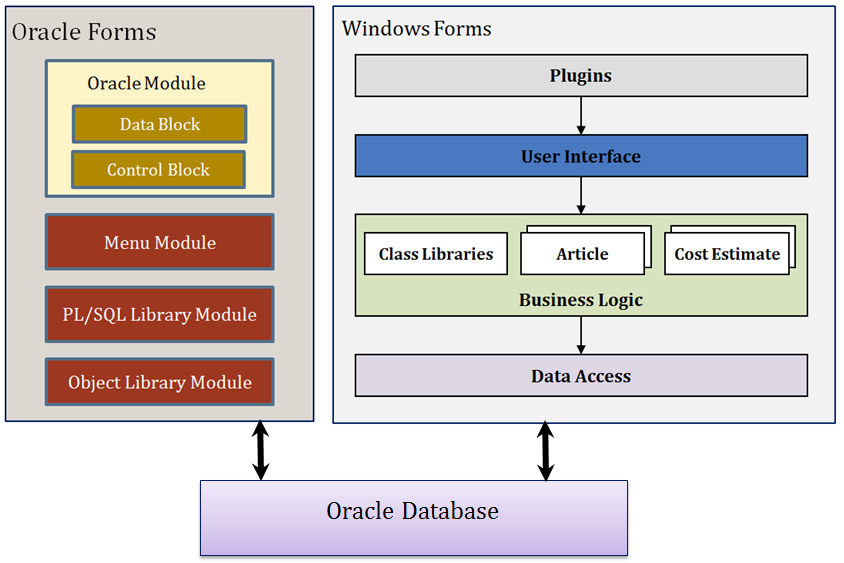
\includegraphics[width=.9\textwidth]{pic_old_new.png}\label{fig_system}
	\caption{Old and new system architecture.}
\end{figure}
\par
The high volume of business rules might be encountered as another drawback in our task. Most of the business rules in the specs cannot be fully understood. Besides, the previous system is provided with some patterns due to the view of the designers at that time. The growth speed of the business requirements soon far exceeds the designers' vision. The code base cannot adapt all the variety of requirements. The previous patterns designed in order to support extensibility and scale up seems to be obsolete in this situation. Our customer showed their interests in the CSLA, Windows form and NHibernate technologies. We marked down this and focus on these technologies to build up our new application. The new application must strictly follow the specs delivered by our company. We as a team of five developers will organize and create the module in the period of three weeks which will be called a spint'' (please refer to figure \ref{fig_sprint} in the next page for an illustration). Every three weeks, we receive a set of task sheets. They are modules that we are going to implement. We first read the specs relevant to the delivered task sheets carefully. The implementation starts from the lowest level of the system architecture, which is the database. We might write the database script if there is any necessary change in the database to conform the module described in the task sheet. We then implement the data access layer. After that, we implement the business layer and then the GUI. Our last step is to test and fix the bugs if there is any. The last step is to optimize the functions and code. This is our typical routine in finishing a task in a spint. We have to strictly follow the company architecture.  The architecture will be described in chapter 3 because understanding and being able to follow the architecture will lead to the succeed in implementing a new module. 

\begin{sidewaysfigure}
	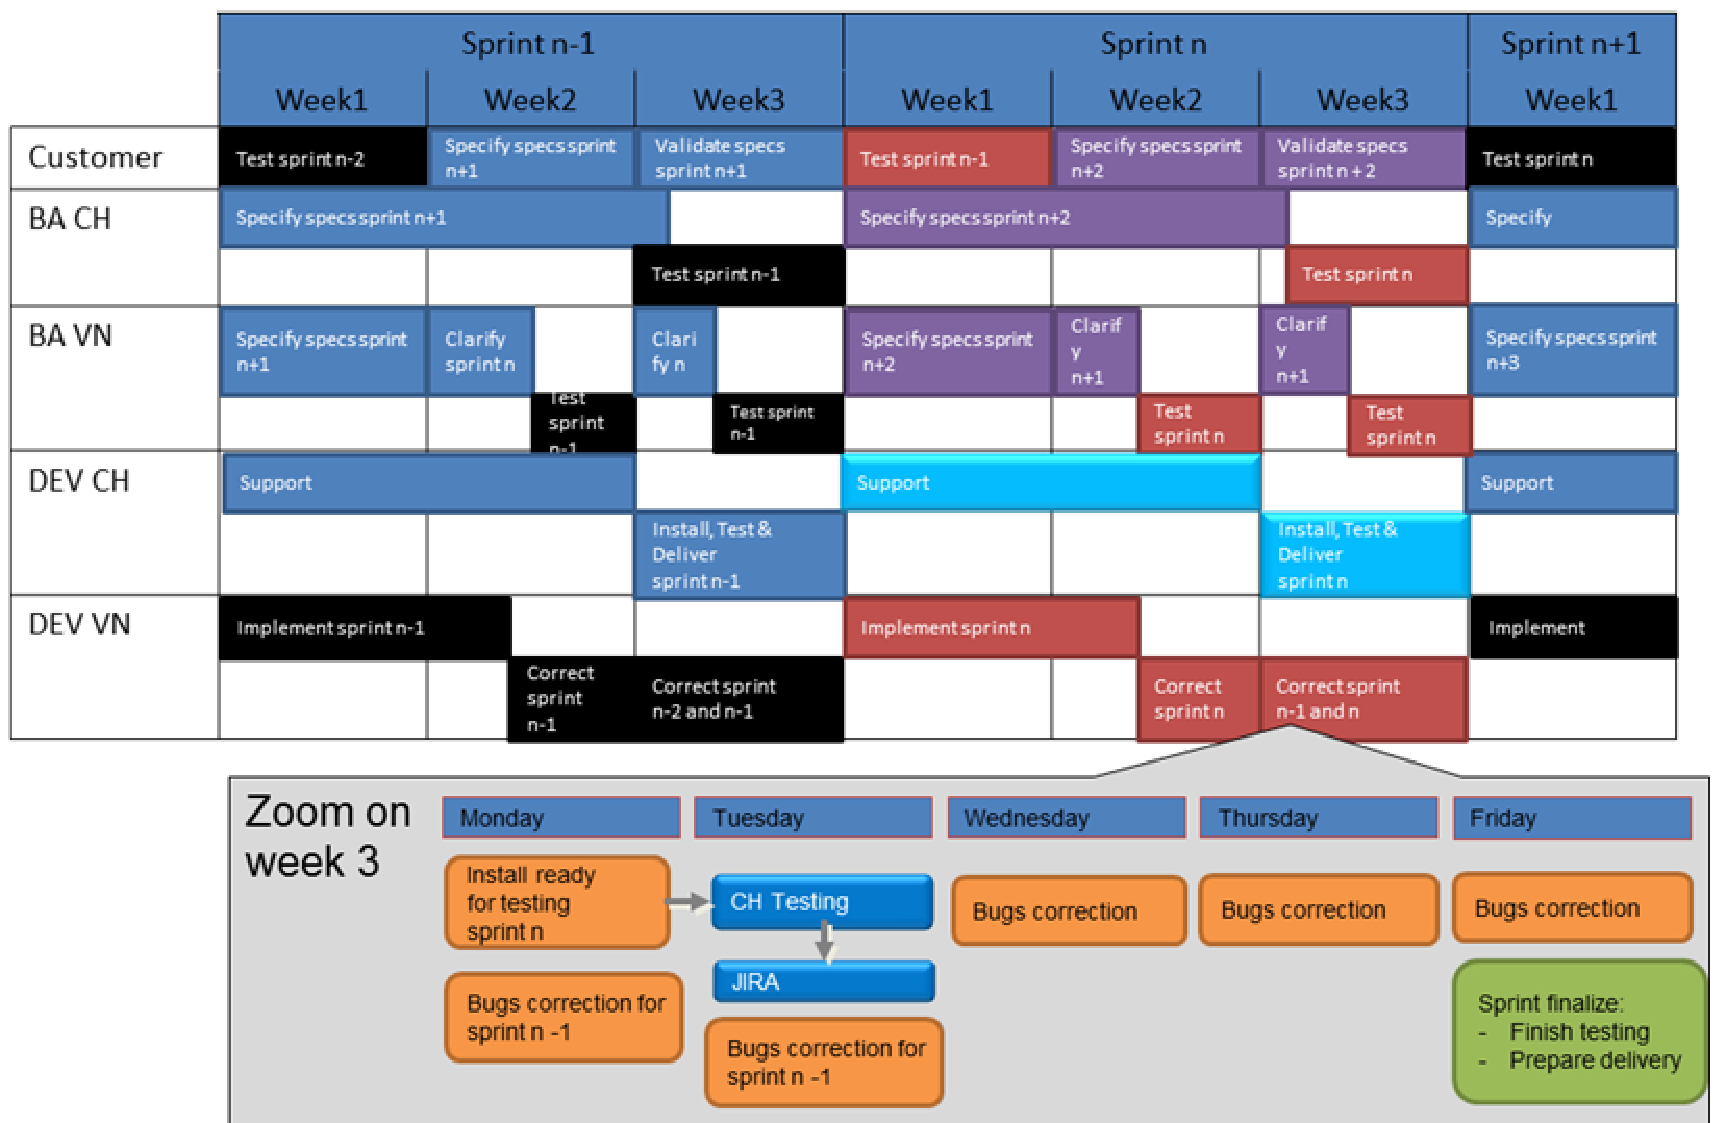
\includegraphics[width=.85\textwidth]{pic_sprint.pdf}
	\caption{An illustration of Sprints} \label{fig_sprint}
	\begin{minipage}[c]{0.5\textwidth}
		BA: business analyst's task\\
		DEV: developers' task	
	\end{minipage}	
	\begin{minipage}[c]{0.5\textwidth}
		CH: task will be done in Switzerland\\
		VN: task will be finished in VietNam
	\end{minipage}	
\end{sidewaysfigure}
\par
Quality Assurance keeps a high priority in our tasks. All of our code must pass a strictly double checked in both VietNam and Switzerland.  The code must first pass the unit test provided by the specs then the test made by our dedicated testers, this phase will be done in three-week time. The successful code will be delivered to the Swiss colleagues for further checked at the fourth week of a sprint.
%

\section{Challenges}\label{sec:challenges}
I found myself a big gap because of the missing experience in CSLA.NET (Component-based Scalable Logical Architecture) and the NHibernate. In the other hand, the application's library is large and is not fully documented. 
\par
The old version of the application, as mentioned previously, is using the Oracle database, we found keys problems with this type of database in migrating. Despite of the Oracle fully supported keys and constraints, there is no foreign key and uniqueness constraints found in this version of the application. We might blame the poor designs of the previous version of the database but this became one of our most concerns in the new design. We must carefully handle this problem due to the fact that foreign key cannot be added in the new version of our application but the new version must persist the data consistency. Besides, the uniqueness constraints are checked using the hard code, which is not recommended in the modern application. We also found many composite keys in this database design which is hard to optimize for NHibernate lazy load as they are designed for.
\par
The old version used package store procedure and native query. The new version is recommended to use the Query Over to generate the query since it is easy to maintain. The problem is that the generated query might not always gives the same results as the previous native queries. The performance is also affected when using the old fashioned native query. In the other hand, the sophisticated queries can only be used in native query. 
\par
Never before did I work with the real system then the high volume of data is another problem occurred. The system also consists of large amount of modules and it takes quite long time to build and debug.
\par
As previous mentioned, all the specs and the schedule must be strictly followed. The specs documents are all business requirements. We as the developers will work with the technical requirements and there are some mismatches in the architecture and design document~\cite{ADD}. 
\par
The main idea of the CSLA is the Parent-child relationship. To take the full advantage of the CSLA, the data model must be mapped into the parent-child relationship. More about this relationship will be described in the book~\cite{EBO, UCS}.
%